\documentclass[t]{beamer}

\usetheme{metropolis}

\author{Esten H{\o}yland Leonardsen}
\date{31.08.22}
\title{Detecting individual-level deviations in brain morphology in MCI patients}

% TIKZ PACKAGES
\usetikzlibrary{arrows.meta}
\usetikzlibrary{calc}

% COLOUR
\definecolor{cb-pink}{HTML}{eeafcf}
\definecolor{cb-orange}{HTML}{e59145}
\definecolor{cb-light-brown}{HTML}{baa066}
\definecolor{cb-blue}{HTML}{3594d6}
\definecolor{cb-green}{HTML}{4dac93}
\definecolor{cb-gray}{HTML}{3a5c7d}
\definecolor{cb-light-purple}{HTML}{b45899}
\definecolor{cb-red-purple}{HTML}{c71555}
\definecolor{cb-brown}{HTML}{840000}
\definecolor{cb-blue-purple}{HTML}{662fa2}

\begin{document}
	\titlepage
	\begin{frame}{Explainable AI}
		\begin{tikzpicture}

			\newcommand{\nodesize}{11pt}
			\newcommand{\hsep}{28pt}
			\newcommand{\vsep}{14pt}

			\newcommand{\arrowwidth}{0.05cm}
			\newcommand{\innerarrow}{{Latex[length=0.1cm, width=0.15cm]}}
			\newcommand{\outerarrow}{{Latex[length=0.2cm, width=0.3cm]}}

			\newcommand{\mrilocation}[1]{($(1, -2.2)$)}
			\newcommand{\modellocation}[1]{($ (0.5 * 11, -2.2) + ####1 $)}
			\newcommand{\lrplocation}[1]{($ (0.5 * 11, -5.2) + ####1 $)}


			\def\maplocation{(1, -5.2)}

			\newcommand{\mrialpha}{0.2}
			\definecolor{outercolor}{RGB}{128, 128, 128}
			\colorlet{predict-fill}{cb-blue}
			\colorlet{lrp-fill}{red}

			\node[inner sep=0pt, outer sep=0pt] (input) at \mrilocation{(0, 0)} {
				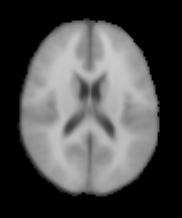
\includegraphics[height=0.5cm]{data/slice.png}
			};

			\node[circle, inner sep=0pt, fill=none, outer sep=0pt, line width=0pt, draw=none] (n00) at \modellocation{(-3 * \hsep, 0)} {};

			\node[circle, minimum size=\nodesize, inner sep=0pt, fill=predict-fill!85, outer sep=0pt, line width=0pt, draw=predict-fill!85] (n10) at \modellocation{(-2 * \hsep, 2 * \vsep)} {};
			\node[circle, minimum size=\nodesize, inner sep=0pt, fill=predict-fill, outer sep=0pt, line width=0pt, draw=predict-fill] (n11) at \modellocation{(-2 * \hsep, 1 * \vsep)} {};
			\node[circle, minimum size=\nodesize, inner sep=0pt, fill=predict-fill!75, outer sep=0pt, line width=0pt, draw=predict-fill!75] (n12) at \modellocation{(-2 * \hsep, 0)} {};
			\node[circle, minimum size=\nodesize, inner sep=0pt, fill=predict-fill!15, outer sep=0pt, line width=0pt, draw=predict-fill!15] (n13) at \modellocation{(-2 * \hsep, -1 * \vsep)} {};
			\node[circle, minimum size=\nodesize, inner sep=0pt, fill=predict-fill!50, outer sep=0pt, line width=0pt, draw=predict-fill!50] (n14) at \modellocation{(-2 * \hsep, -2 * \vsep)} {};

			\node[circle, minimum size=\nodesize, inner sep=0pt, fill=predict-fill!15, outer sep=0pt, line width=0pt, draw=predict-fill!15] (n20) at \modellocation{(-1 * \hsep, 1.5 * \vsep)} {};
			\node[circle, minimum size=\nodesize, inner sep=0pt, fill=predict-fill!65, outer sep=0pt, line width=0pt, draw=predict-fill!65] (n21) at \modellocation{(-1 * \hsep, 0.5 * \vsep)} {};
			\node[circle, minimum size=\nodesize, inner sep=0pt, fill=predict-fill!90, outer sep=0pt, line width=0pt, draw=predict-fill!90] (n22) at \modellocation{(-1 * \hsep, -0.5 * \vsep)} {};
			\node[circle, minimum size=\nodesize, inner sep=0pt, fill=predict-fill!40, outer sep=0pt, line width=0pt, draw=predict-fill!40] (n23) at \modellocation{(-1 * \hsep, -1.5 * \vsep)} {};

			\node[circle, minimum size=\nodesize, inner sep=0pt, fill=predict-fill!80, outer sep=0pt, line width=0pt, draw=predict-fill!80] (n30) at \modellocation{(0 * \hsep, 1.5 * \vsep)} {};
			\node[circle, minimum size=\nodesize, inner sep=0pt, fill=predict-fill!55, outer sep=0pt, line width=0pt, draw=predict-fill!55] (n31) at \modellocation{(0 * \hsep, 0.5 * \vsep)} {};
			\node[circle, minimum size=\nodesize, inner sep=0pt, fill=predict-fill!15, outer sep=0pt, line width=0pt, draw=predict-fill!15] (n32) at \modellocation{(0 * \hsep, -0.5 * \vsep)} {};
			\node[circle, minimum size=\nodesize, inner sep=0pt, fill=predict-fill!75, outer sep=0pt, line width=0pt, draw=predict-fill!75] (n33) at \modellocation{(0 * \hsep, -1.5 * \vsep)} {};

			\node[circle, minimum size=\nodesize, inner sep=0pt, fill=predict-fill, outer sep=0pt, line width=0pt, draw=predict-fill] (n40) at \modellocation{(1 * \hsep, 1*\vsep)} {};
			\node[circle, minimum size=\nodesize, inner sep=0pt, fill=predict-fill!20, outer sep=0pt, line width=0pt, draw=predict-fill!20] (n41) at \modellocation{(1 * \hsep, 0*\vsep)} {};
			\node[circle, minimum size=\nodesize, inner sep=0pt, fill=predict-fill!15, outer sep=0pt, line width=0pt, draw=predict-fill!15] (n42) at \modellocation{(1 * \hsep, -1*\vsep)} {};

			\node[circle, minimum size=\nodesize, inner sep=0pt, fill=predict-fill!75, outer sep=0pt, line width=0pt, draw=predict-fill!75] (n50) at \modellocation{(2 * \hsep, 1*\vsep)} {};
			\node[circle, minimum size=\nodesize, inner sep=0pt, fill=predict-fill!35, outer sep=0pt, line width=0pt, draw=predict-fill!35] (n51) at \modellocation{(2 * \hsep, 0*\vsep)} {};
			\node[circle, minimum size=\nodesize, inner sep=0pt, fill=predict-fill!65, outer sep=0pt, line width=0pt, draw=predict-fill!65] (n52) at \modellocation{(2 * \hsep, -1*\vsep)} {};

			\node[circle, minimum size=\nodesize, inner sep=0pt, fill=predict-fill!85, outer sep=0pt, line width=0pt, draw=predict-fill!85] (output) at \modellocation{(3 * \hsep, 0)} {};

			\node[] (diagnosis) at (1+2*4.85, -2.2) {\scriptsize{prediction}};

			\draw[
				color=predict-fill!85,
				-\innerarrow,
				line width=\arrowwidth
			] (n00) to [out=20,in=200] (n10) {};
			\draw[
				color=predict-fill,
				-\innerarrow,
				line width=\arrowwidth
			] (n00) to [out=10,in=190] (n11) {};
			\draw[
				color=predict-fill!75,
				-\innerarrow,
				line width=\arrowwidth
			] (n00) to [out=0,in=180] (n12) {};
			\draw[
				color=predict-fill!15,
				-\innerarrow,
				line width=\arrowwidth
			] (n00) to [out=-10,in=170] (n13) {};
			\draw[
				color=predict-fill!50,
				-\innerarrow,
				line width=\arrowwidth
			] (n00) to [out=-20,in=160] (n14) {};

			\draw[
				color=predict-fill!75,
				-\innerarrow,
				line width=\arrowwidth
			] (n10) to [out=-5,in=175] (n20) {};
			\draw[
				color=predict-fill!50,
				-\innerarrow,
				line width=\arrowwidth
			] (n10) to [out=-15,in=165] (n21) {};
			\draw[
				color=predict-fill!55,
				-\innerarrow,
				line width=\arrowwidth
			] (n10) to [out=-25,in=155] (n22) {};
			\draw[
				color=predict-fill!85,
				-\innerarrow,
				line width=\arrowwidth
			] (n10) to [out=-35,in=145] (n23) {};

			\draw[
				color=predict-fill!45,
				-\innerarrow,
				line width=\arrowwidth
			] (n11) to [out=5,in=185] (n20) {};
			\draw[
				color=predict-fill!50,
				-\innerarrow,
				line width=\arrowwidth
			] (n11) to [out=-5,in=175] (n21) {};
			\draw[
				color=predict-fill,
				-\innerarrow,
				line width=\arrowwidth
			] (n11) to [out=-15,in=165] (n22) {};
			\draw[
				color=predict-fill!15,
				-\innerarrow,
				line width=\arrowwidth
			] (n11) to [out=-25,in=155] (n23) {};

			\draw[
				color=predict-fill!35,
				-\innerarrow,
				line width=\arrowwidth
			] (n12) to [out=15,in=195] (n20) {};
			\draw[
				color=predict-fill!90,
				-\innerarrow,
				line width=\arrowwidth
			] (n12) to [out=5,in=185] (n21) {};
			\draw[
				color=predict-fill!80,
				-\innerarrow,
				line width=\arrowwidth
			] (n12) to [out=-5,in=175] (n22) {};
			\draw[
				color=predict-fill!20,
				-\innerarrow,
				line width=\arrowwidth
			] (n12) to [out=-15,in=165] (n23) {};

			\draw[
				color=predict-fill!55,
				-\innerarrow,
				line width=\arrowwidth
			] (n13) to [out=25,in=205] (n20) {};
			\draw[
				color=predict-fill!65,
				-\innerarrow,
				line width=\arrowwidth
			] (n13) to [out=15,in=195] (n21) {};
			\draw[
				color=predict-fill!35,
				-\innerarrow,
				line width=\arrowwidth
			] (n13) to [out=5,in=185] (n22) {};
			\draw[
				color=predict-fill!45,
				-\innerarrow,
				line width=\arrowwidth
			] (n13) to [out=-5,in=175] (n23) {};

			\draw[
				color=predict-fill!10,
				-\innerarrow,
				line width=\arrowwidth
			] (n14) to [out=35,in=215] (n20) {};
			\draw[
				color=predict-fill!90,
				-\innerarrow,
				line width=\arrowwidth
			] (n14) to [out=25,in=205] (n21) {};
			\draw[
				color=predict-fill!80,
				-\innerarrow,
				line width=\arrowwidth
			] (n14) to [out=15,in=195] (n22) {};
			\draw[
				color=predict-fill!35,
				-\innerarrow,
				line width=\arrowwidth
			] (n14) to [out=5,in=185] (n23) {};

			\draw[
				color=predict-fill!75,
				-\innerarrow,
				line width=\arrowwidth
			] (n20) to [out=0,in=180] (n30) {};
			\draw[
				color=predict-fill!50,
				-\innerarrow,
				line width=\arrowwidth
			] (n20) to [out=-10,in=170] (n31) {};
			\draw[
				color=predict-fill!85,
				-\innerarrow,
				line width=\arrowwidth
			] (n20) to [out=-20,in=160] (n32) {};
			\draw[
				color=predict-fill!45,
				-\innerarrow,
				line width=\arrowwidth
			] (n20) to [out=-30,in=150] (n33) {};

			\draw[
				color=predict-fill!20,
				-\innerarrow,
				line width=\arrowwidth
			] (n21) to [out=10,in=190] (n30) {};
			\draw[
				color=predict-fill!35,
				-\innerarrow,
				line width=\arrowwidth
			] (n21) to [out=0,in=180] (n31) {};
			\draw[
				color=predict-fill!15,
				-\innerarrow,
				line width=\arrowwidth
			] (n21) to [out=-10,in=170] (n32) {};
			\draw[
				color=predict-fill!90,
				-\innerarrow,
				line width=\arrowwidth
			] (n21) to [out=-20,in=160] (n33) {};

			\draw[
				color=predict-fill!65,
				-\innerarrow,
				line width=\arrowwidth
			] (n22) to [out=20,in=200] (n30) {};
			\draw[
				color=predict-fill!20,
				-\innerarrow,
				line width=\arrowwidth
			] (n22) to [out=10,in=190] (n31) {};
			\draw[
				color=predict-fill!30,
				-\innerarrow,
				line width=\arrowwidth
			] (n22) to [out=0,in=180] (n32) {};
			\draw[
				color=predict-fill!40,
				-\innerarrow,
				line width=\arrowwidth
			] (n22) to [out=-10,in=170] (n33) {};

			\draw[
				color=predict-fill,
				-\innerarrow,
				line width=\arrowwidth
			] (n23) to [out=30,in=210] (n30) {};
			\draw[
				color=predict-fill!15,
				-\innerarrow,
				line width=\arrowwidth
			] (n23) to [out=20,in=200] (n31) {};
			\draw[
				color=predict-fill!75,
				-\innerarrow,
				line width=\arrowwidth
			] (n23) to [out=10,in=190] (n32) {};
			\draw[
				color=predict-fill!35,
				-\innerarrow,
				line width=\arrowwidth
			] (n23) to [out=0,in=180] (n33) {};

			\draw[
				color=predict-fill!70,
				-\innerarrow,
				line width=\arrowwidth
			] (n30) to [out=-5,in=175] (n40) {};
			\draw[
				color=predict-fill!80,
				-\innerarrow,
				line width=\arrowwidth
			] (n30) to [out=-15,in=165] (n41) {};
			\draw[
				color=predict-fill!20,
				-\innerarrow,
				line width=\arrowwidth
			] (n30) to [out=-25,in=155] (n42) {};

			\draw[
				color=predict-fill!60,
				-\innerarrow,
				line width=\arrowwidth
			] (n31) to [out=5,in=185] (n40) {};
			\draw[
				color=predict-fill!95,
				-\innerarrow,
				line width=\arrowwidth
			] (n31) to [out=-5,in=175] (n41) {};
			\draw[
				color=predict-fill!35,
				-\innerarrow,
				line width=\arrowwidth
			] (n31) to [out=-15,in=165] (n42) {};

			\draw[
				color=predict-fill!75,
				-\innerarrow,
				line width=\arrowwidth
			] (n32) to [out=15,in=195] (n40) {};
			\draw[
				color=predict-fill!20,
				-\innerarrow,
				line width=\arrowwidth
			] (n32) to [out=5,in=185] (n41) {};
			\draw[
				color=predict-fill!15,
				-\innerarrow,
				line width=\arrowwidth
			] (n32) to [out=-5,in=175] (n42) {};

			\draw[
				color=predict-fill!40,
				-\innerarrow,
				line width=\arrowwidth
			] (n33) to [out=25,in=205] (n40) {};
			\draw[
				color=predict-fill!80,
				-\innerarrow,
				line width=\arrowwidth
			] (n33) to [out=15,in=195] (n41) {};
			\draw[
				color=predict-fill!50,
				-\innerarrow,
				line width=\arrowwidth
			] (n33) to [out=5,in=185] (n42) {};

			\draw[
				color=predict-fill!25,
				-\innerarrow,
				line width=\arrowwidth
			] (n40) to [out=0,in=180] (n50) {};
			\draw[
				color=predict-fill!50,
				-\innerarrow,
				line width=\arrowwidth
			] (n40) to [out=-10,in=170] (n51) {};
			\draw[
				color=predict-fill!45,
				-\innerarrow,
				line width=\arrowwidth
			] (n40) to [out=-20,in=160] (n52) {};

			\draw[
				color=predict-fill!90,
				-\innerarrow,
				line width=\arrowwidth
			] (n41) to [out=10,in=190] (n50) {};
			\draw[
				color=predict-fill!10,
				-\innerarrow,
				line width=\arrowwidth
			] (n41) to [out=0,in=180] (n51) {};
			\draw[
				color=predict-fill!75,
				-\innerarrow,
				line width=\arrowwidth
			] (n41) to [out=-10,in=170] (n52) {};

			\draw[
				color=predict-fill!60,
				-\innerarrow,
				line width=\arrowwidth
			] (n42) to [out=20,in=200] (n50) {};
			\draw[
				color=predict-fill!25,
				-\innerarrow,
				line width=\arrowwidth
			] (n42) to [out=10,in=190] (n51) {};
			\draw[
				color=predict-fill!15,
				-\innerarrow,
				line width=\arrowwidth
			] (n42) to [out=0,in=180] (n52) {};

			\draw[
				color=predict-fill!95,
				-\innerarrow,
				line width=\arrowwidth
			] (n50) to [out=-10,in=170] (output) {};
			\draw[
				color=predict-fill!25,
				-\innerarrow,
				line width=\arrowwidth
			] (n51) to [out=0,in=180] (output) {};
			\draw[
				color=predict-fill!50,
				-\innerarrow,
				line width=\arrowwidth
			] (n52) to [out=10,in=190] (output) {};

			\draw[black] (n00.center) --
						 ($ (n00) + (0, 2*\vsep+0.5*\nodesize+2pt) $) --
						 ($ (n00) + (6*\hsep+0.5*\nodesize+2pt, 2*\vsep+0.5*\nodesize+2pt) $) --
						 ($ (n00) + (6*\hsep+0.5*\nodesize+2pt, -2*\vsep-0.5*\nodesize-2pt) $) --
						 ($ (n00) + (0, -2*\vsep-0.5*\nodesize-2pt) $) -- (n00.center);

			\node[] at ($ (n30) + (0, \vsep+0.5*\nodesize) $) {\footnotesize{CNN}};

			\draw[
				color=outercolor,
				-\outerarrow,
				line width=0.1cm
			] (input) to [out=0,in=180] (n00) {};
			\draw[
				color=outercolor,
				-\outerarrow,
				line width=0.1cm
			] (output) to [out=0,in=180] (diagnosis) {};
		\end{tikzpicture}
	\end{frame}
\end{document}
